\documentclass[border=0.8ex,svgnames,tikz]{standalone}
\usepackage{amsmath,mathtools}
\usepackage{fontspec}
\setmainfont{Source Serif 4}
\setsansfont{Source Sans 3}
\setmonofont{Source Code Pro}

\usetikzlibrary{chains}

\begin{document}
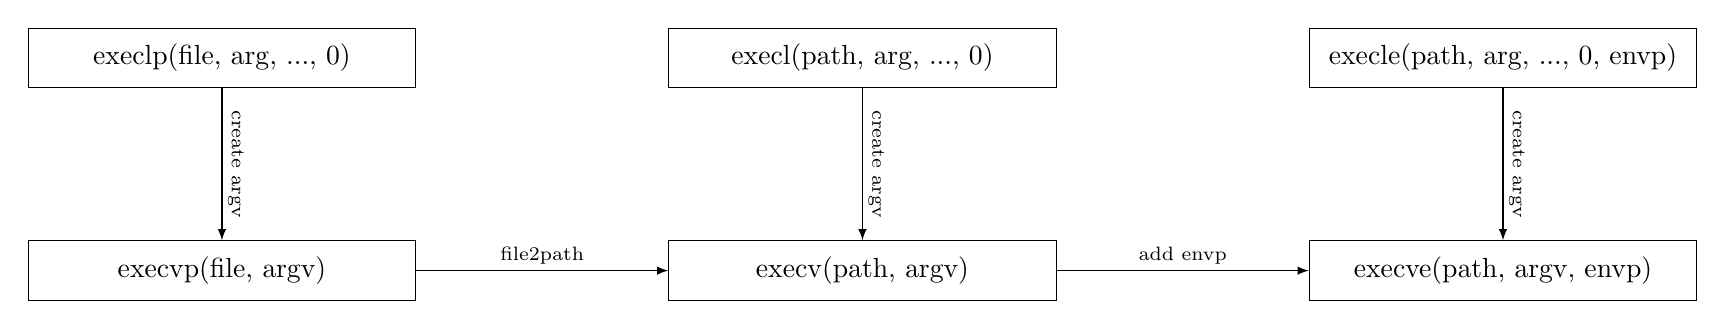
\begin{tikzpicture}
  \coordinate (familyl-start) at (0.0,2.7);
  \coordinate (familyv-start) at (0.0,0.0);
  \begin{scope}[
    every node/.style={
      draw,
      on chain,
      minimum width=14em,
      minimum height=5ex,
      font=\normalsize,
    },
    node distance=3.2,
    start chain=going right,
    ]
    \chainin (familyl-start);
    \node (execlp) {execlp(file, arg, ..., 0)};
    \node (execl)  {execl(path, arg, ..., 0)};
    \node (execle) {execle(path, arg, ..., 0, envp)};
    \chainin (familyv-start);
    \node (execvp) {execvp(file, argv)};
    \node (execv)  {execv(path, argv)};
    \node (execve) {execve(path, argv, envp)};
  \end{scope}
  \begin{scope}[
    every node/.style={inner sep=2pt,above,sloped,font=\scriptsize},
    every path/.style={draw,-latex},
    ]
    \path
    (execlp) edge node{create argv} (execvp)
    (execl)  edge node{create argv} (execv)
    (execle) edge node{create argv} (execve)
    (execvp) edge node{file2path}   (execv)
    (execv)  edge node{add envp}    (execve);
    \end{scope}
\end{tikzpicture}
\end{document}
